\documentclass[11pt]{article}
\usepackage[margin=1in]{geometry}
\usepackage{enumerate}
\usepackage{framed}
\usepackage{multirow}
\usepackage{multicol}
\usepackage{bm}
\usepackage{amssymb}
\usepackage{amsmath}
\usepackage{amsthm}
\usepackage{multicol}
\usepackage{graphicx}
\usepackage{float}
\usepackage{hyperref}
\hypersetup{    
    colorlinks=true,
    urlcolor=blue
}
\setlength{\columnsep}{1in}
\begin{document}
\begin{center}
  \begin{tabular}{ | l | p{125mm} |  }
    \hline
    \textbf{Members} &  Savannah Baron and Varsha Kishore \\ \hline
    \textbf{Title} & Predicting Political Ideology \\ \hline
    \textbf{Hours} & Savannah (8), Varsha (8) \\ \hline
    \textbf{Predicting} & Our goal is to classify the political ideology of sentences. In particular, a binary classification problem to start (conservative/liberal) and a three class problem later (conservative/liberal/neutral). \\ \hline
    \textbf{Data} &  We will be using data from the \href{http://cs.umd.edu/~miyyer/ibc/}{Ideological Books Corpus} (IBC). This data set contains sentences from authors with known political standings. All sentences are labeled as either liberal, conservative or neutral. There are 4062 sentences total, with 2025 of them being liberal, 1701 conservative, and 600 neutral. \\ \hline
    \textbf{Features} &  Currently we are using bag of words for our feautres, so our feature space is dependent upon the number of words we choose to use in our vocabulary. We've been experimenting with using between 2000 and all (about 11000) words, and have been experimenting with how to form and select these words in a variety of ways. Some examples of things we have tried so far include removal of stop words, n-grams, using stem words, and Tf-Idf (Term Frequency-Inverse Document Frequency). \\ \hline
    \textbf{Models} & So far, we are focusing on a textual classification problem. So, we are using the ever popular SVM and Logistic Regression models to begin with because these models have been used for other similar textual classification problems. Using Logistic regression also gives us a direct probabilistic interpretation and this might be useful in our analysis. An advantage we have with SVM's is that we can use kernels to encode additional relationships between words. \\ \hline
    \textbf{Results} & \begin{tabular}{|r|p{50mm}|r|r|} \hline
    \textbf{Model} & \textbf{Best Params} & \textbf{Average Accuracy} \\ \hline
    Random & N/A & 50\% \\ \hline
    SVM & Used NLTK to remove stop words, used NLTK to extract words using tokenize, used linear SVM with cost C=10 & About 62\% \\ \hline
    LogReg & Remove English Stop Words, Number of Features $\geq$ 1000, Other features tried make little difference & About 65\% \\ \hline
    \end{tabular}
    \\ \hline
    \textbf{Problems} &  The lone professional paper that uses this dataset achieves a maximum accuracy 69.3\% (using recursive neural nets (RNN)). This is not that great, so whether we'll be able to improve from where we are currently, or beyond that far enough to get interesting results is an open question. Additionally, we don't have a lot of data, which may limit the amount that our model will generalize.  \\ \hline
    \textbf{Future} & We are planning to look into better feature extraction techniques. This includes looking for negation in sentences, n-grams and specifically politically biased n-grams, and \texttt{nltk} chunking which groups parts of sentences. We also plan to pursue multiclass classification to include neutral examples using random forests. Finally, LDA seems as though it may be interesting in conjunction with our supervised models if we used the results as inputs, however tuning the number of topics in LDA is difficult and subjective, so we plan to time box ourselves to 2 hours initially, and evaluate the results. We can also use LDA to examine what words are being classified as liberal and what words are being classified as conservative. \\ \hline
  \end{tabular}
\end{center}

% Split table onto two pages manually because latex is dumb lol
\begin{center}
  \begin{tabular}{ | l | p{125mm} |  }
    \hline
    \textbf{Specific Questions} & We feel like we don't have great intuition on how to improve the accuracy of our models, or what sorts of features will perform best. This is perhaps more of a``how to do machine learning" question than a specific one though. Additionally, we wonder whether there are there other classifiers that we haven't talked about that could give us better results with text classification. \\ \hline
  \end{tabular}
\end{center}

\textbf{Appendix: Example Visualizations:}

ROC Plot For Log Reg with parameters as shown in title using 10-Fold cross validation. Area seems about as one might expect given the average performance of 0.65 found for this model. 

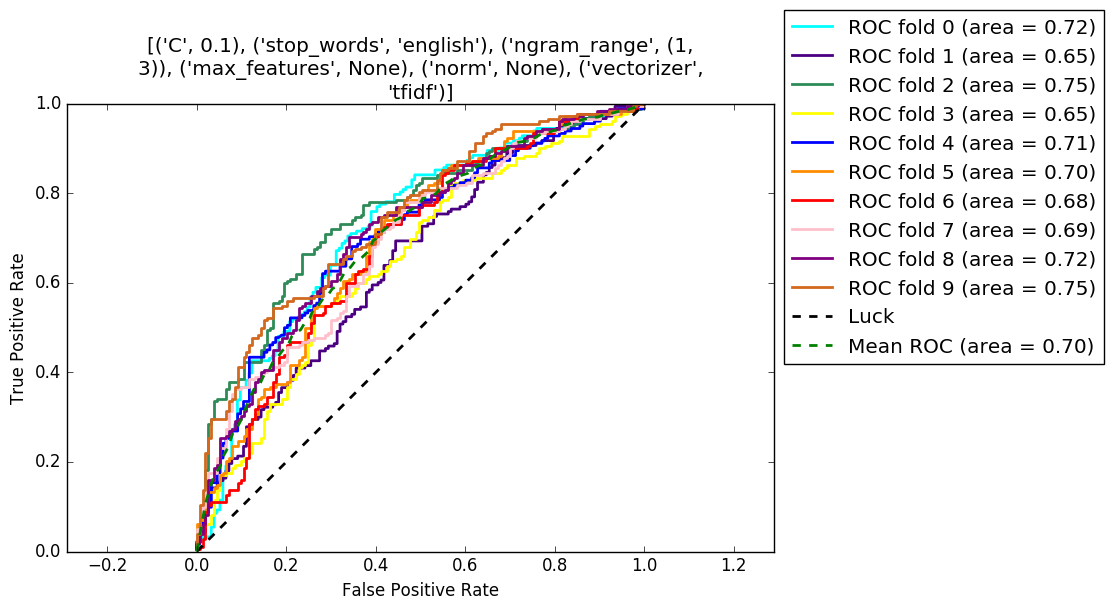
\includegraphics[scale=0.65]{UpdateVis/ROCPlot}

1 of 10 confusion matrices for the same LogReg model as above. For most of the folds including this one, the confusion matrix shows that misclassifications are relatively balanced between the two classes, which is good given that the proportion of the classes is slightly unbalanced in the data. We are using class weights to offset this problem, which does seem to be working.

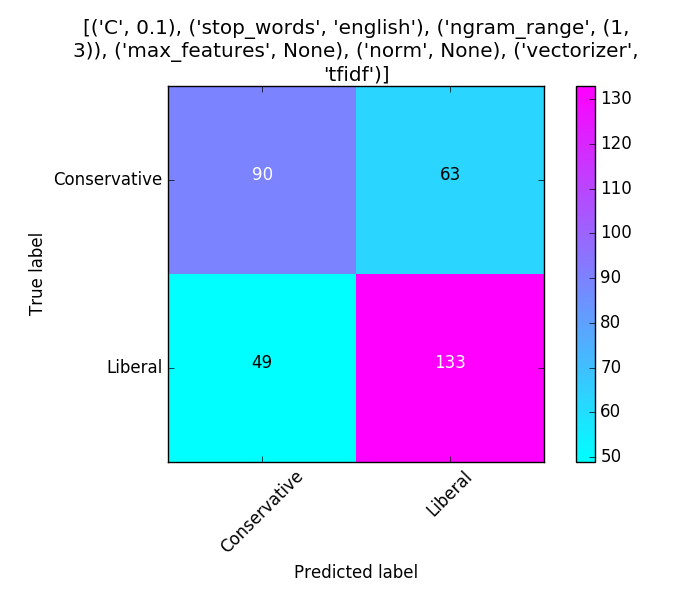
\includegraphics[scale=0.65]{UpdateVis/cm_fold9.png}

\end{document}
